\documentclass[10pt,a4paper]{article}
\usepackage[latin1]{inputenc}
\usepackage{amsmath}
\usepackage{amsfonts}
\usepackage{amssymb}
\usepackage{graphicx}
\usepackage[left=2.00cm, right=2.00cm, bottom=1.00cm, top=1.00cm]{geometry}
\usepackage{subcaption}

\begin{document}
	\begin{figure}
		\caption{Testing}
		\centering
		\begin{subfigure}{0.49\linewidth}
			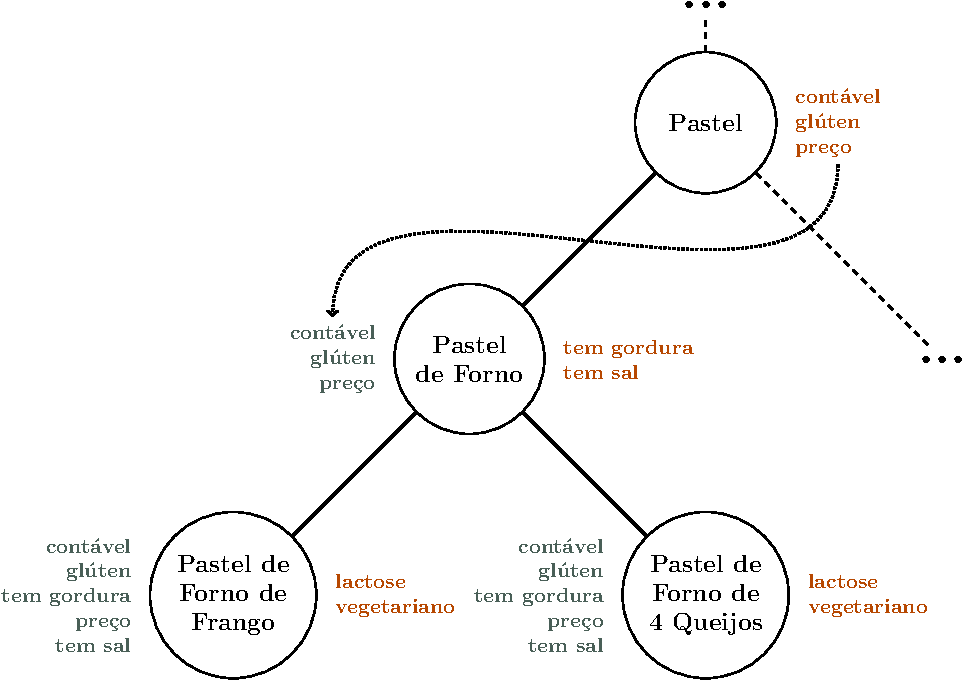
\includegraphics[width=0.9\linewidth]{../topdown-1.pdf}
			\caption{Testing}
		\end{subfigure}
		\begin{subfigure}{0.49\linewidth}
			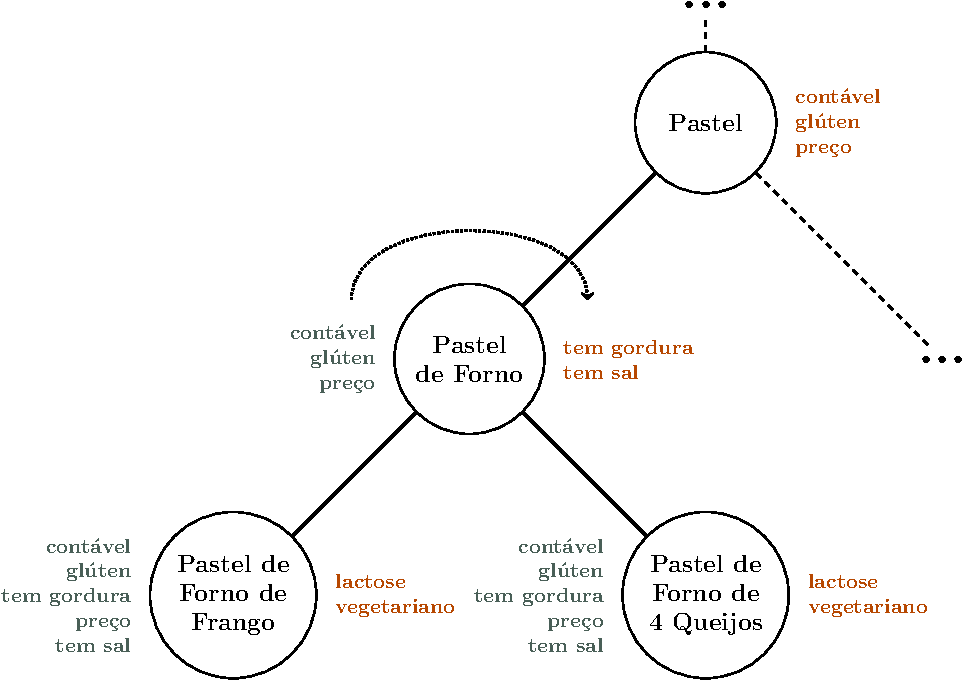
\includegraphics[width=0.9\linewidth]{../topdown-2.pdf}
			\caption{Testing}
		\end{subfigure}
		\\
		\begin{subfigure}{0.49\linewidth}
			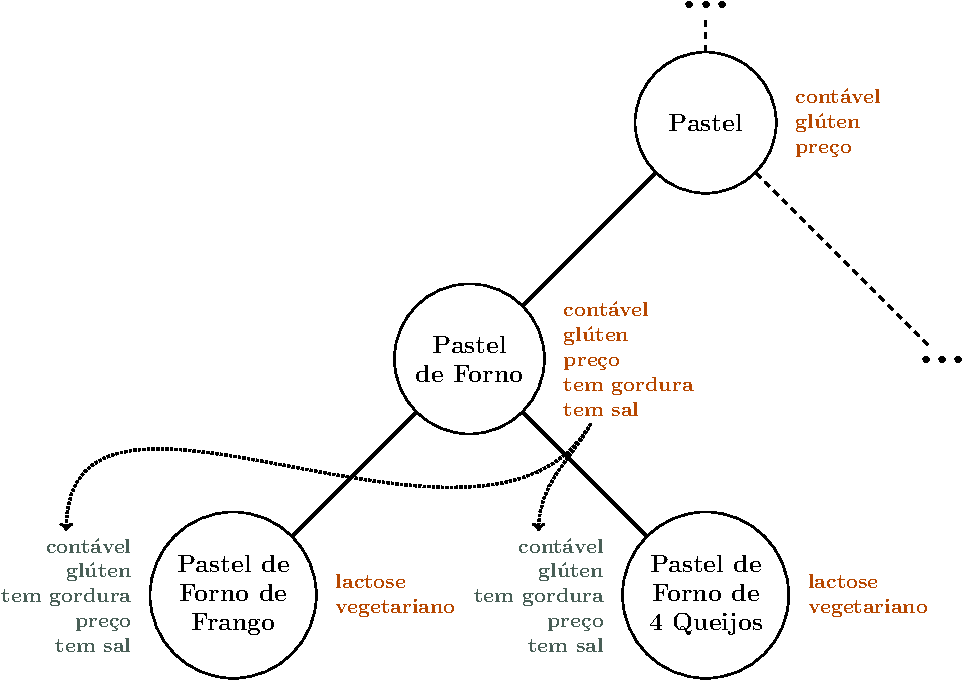
\includegraphics[width=0.9\linewidth]{../topdown-3.pdf}
			\caption{Testing}
		\end{subfigure}
		\begin{subfigure}{0.49\linewidth}
			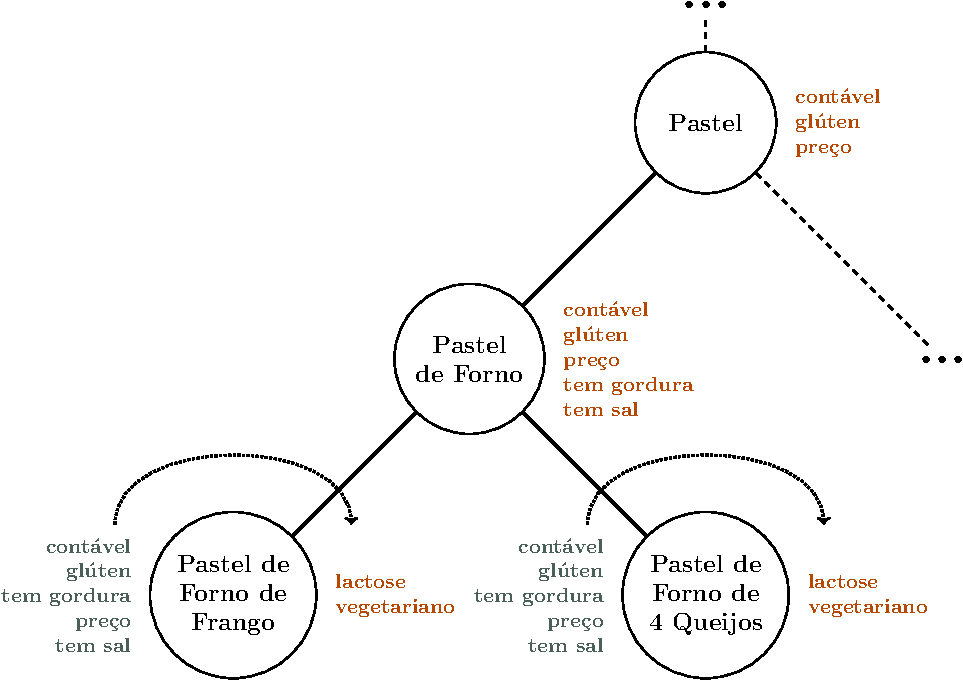
\includegraphics[width=0.9\linewidth]{../topdown-4.pdf}
			\caption{Testing}
		\end{subfigure}
		\\
		\begin{subfigure}{0.49\linewidth}
			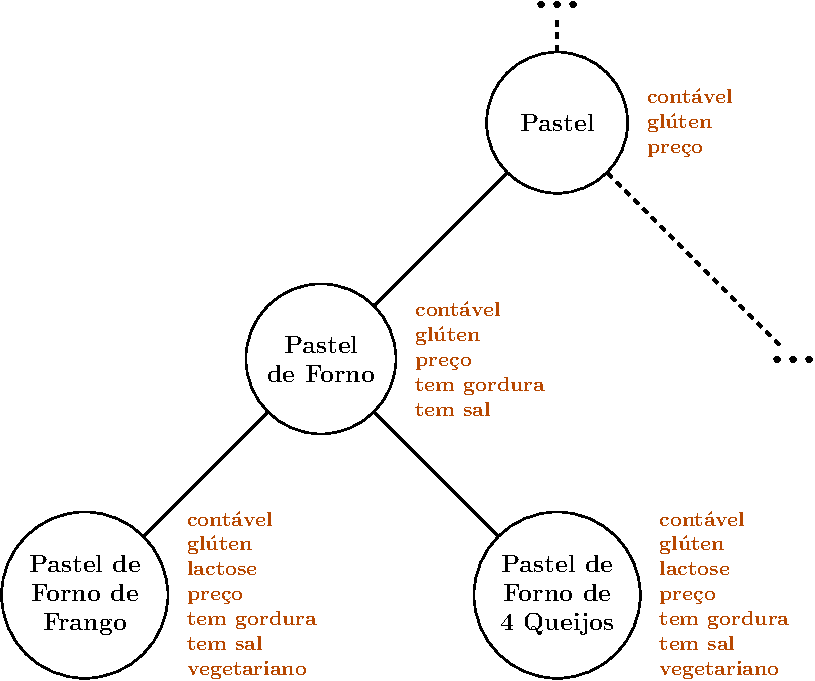
\includegraphics[width=0.9\linewidth]{../topdown-5.pdf}
			\caption{Testing}
		\end{subfigure}
	\end{figure}

	\begin{figure}
		\caption{Testing}
		\centering
		\begin{subfigure}{0.49\linewidth}
			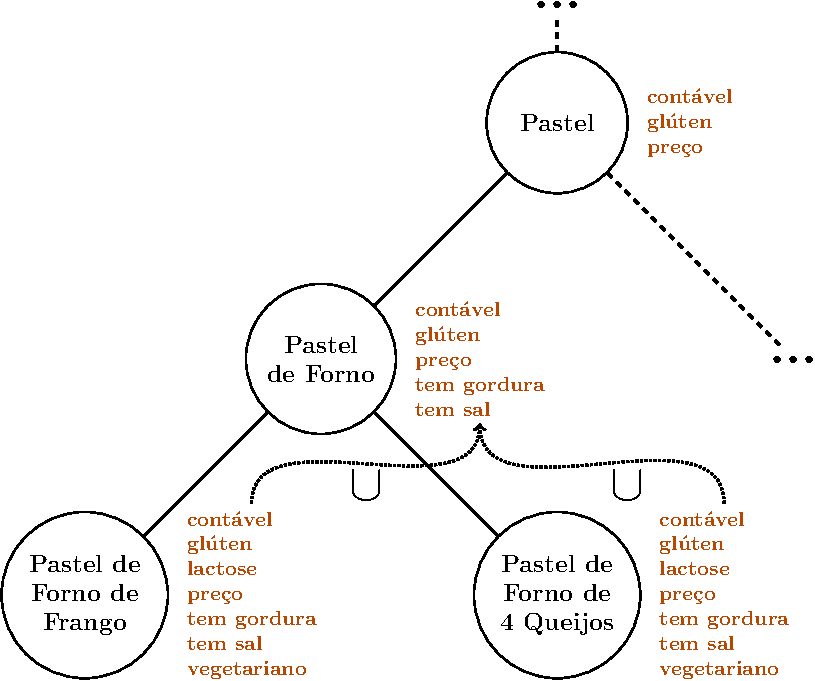
\includegraphics[width=0.9\linewidth]{../bottomup-1.pdf}
			\caption{Testing}
		\end{subfigure}
		\begin{subfigure}{0.49\linewidth}
			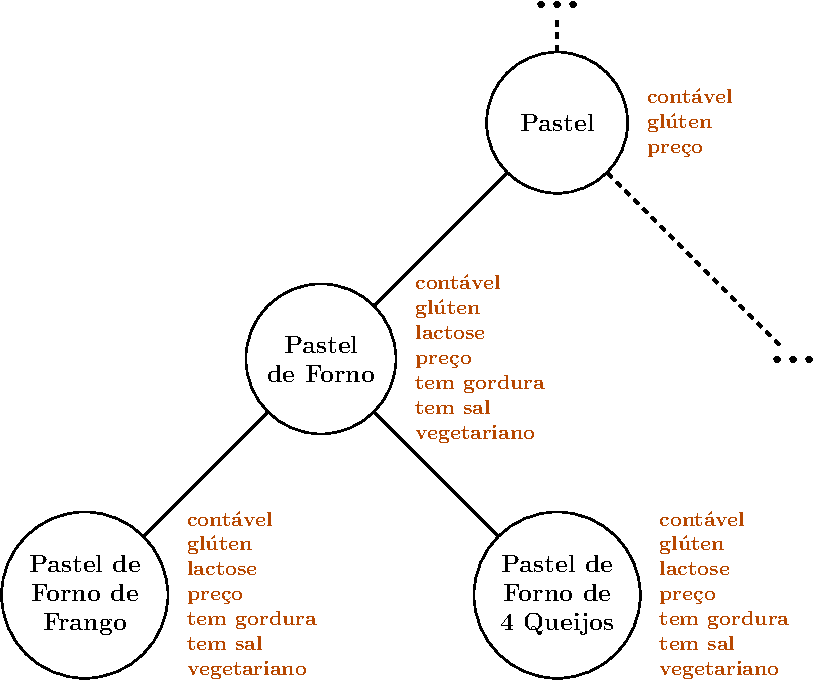
\includegraphics[width=0.9\linewidth]{../bottomup-2.pdf}
			\caption{Testing}
		\end{subfigure}
		\\
		\begin{subfigure}{0.49\linewidth}
			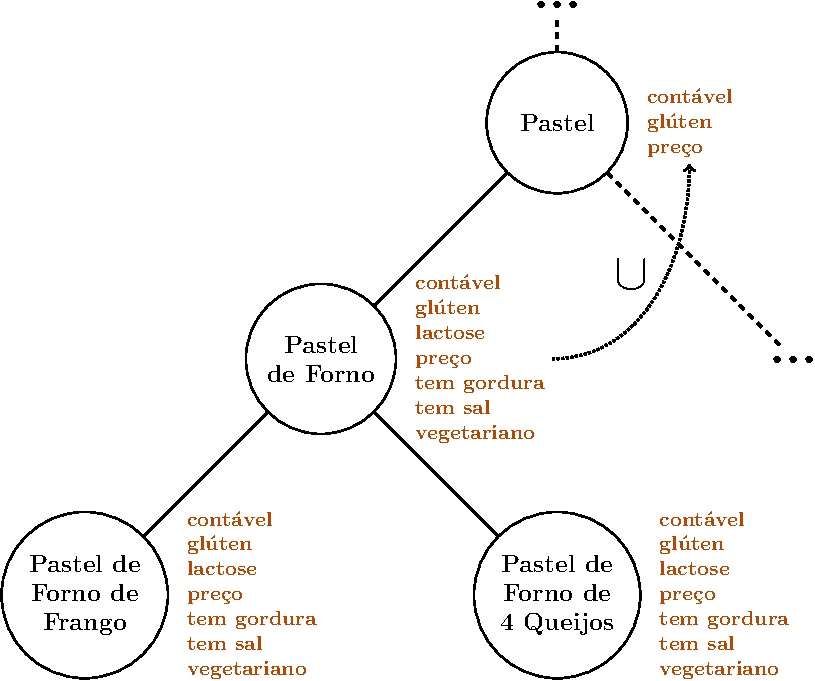
\includegraphics[width=0.9\linewidth]{../bottomup-3.pdf}
			\caption{Testing}
		\end{subfigure}
		\begin{subfigure}{0.49\linewidth}
			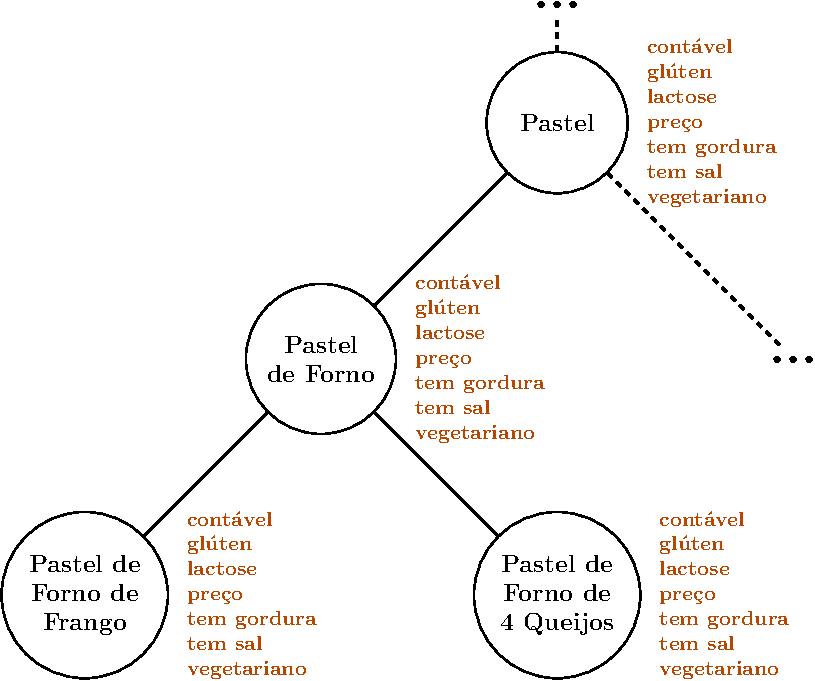
\includegraphics[width=0.9\linewidth]{../bottomup-4.pdf}
			\caption{Testing}
		\end{subfigure}
		\\
		\begin{subfigure}{0.49\linewidth}
			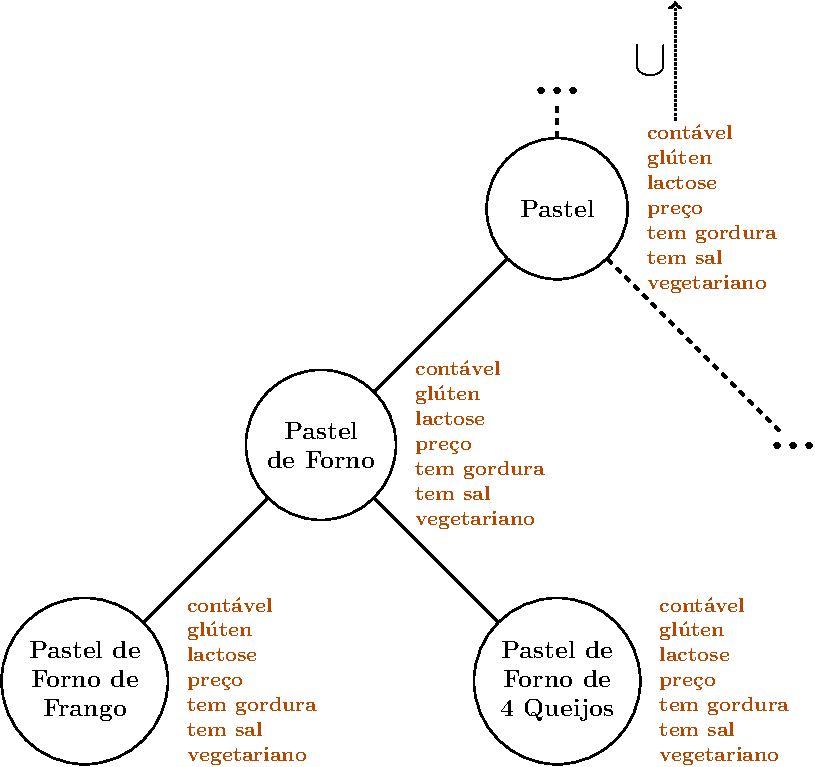
\includegraphics[width=0.9\linewidth]{../bottomup-5.pdf}
			\caption{Testing}
		\end{subfigure}
	\end{figure}
\end{document}